\documentclass[11pt]{article}

\usepackage{ctex}
\usepackage{graphicx}
\usepackage{amsmath, amssymb}
\usepackage{hyperref}
\usepackage{geometry}
\usepackage{listings}
\usepackage{xcolor}
\usepackage{caption}
\usepackage{subcaption}
\usepackage{booktabs}
\geometry{a4paper, margin=1in}

\lstset{
  backgroundcolor=\color{gray!10},
  basicstyle=\ttfamily\small,
  keywordstyle=\color{blue},
  commentstyle=\color{gray},
  stringstyle=\color{orange},
  breaklines=true,
}

\title{\textbf{深度学习导论作业2报告:\\
基于Attention与RNN的垃圾邮件分类模型比较}}
\author{PB22000150 刘行}
\date{2025年4月}

\begin{document}

\maketitle

\tableofcontents

\newpage

\section{实验任务与背景}
本实验基于Enron-Spam数据集, 设计并实现基于自注意力机制 (Multi-head Attention) 与循环神经网络 (RNN) 的文本分类模型, 探究不同架构在垃圾邮件识别任务中的性能表现, 旨在:

\begin{itemize}
	\item 熟悉文本分类任务中的数据清洗、词表构建及编码方法;
	\item 实现具备因果掩码 (Causal Mask) 的自回归多头注意力分类器;
	\item 搭建支持RNN、LSTM、GRU三种变体的循环神经网络分类器;
	\item 系统对比Attention与RNN两类模型在准确率、训练与推理效率上的优劣差异;
	\item 结合注意力权重可视化, 深入理解模型的决策依据与内部机制.
\end{itemize}

\section{数据处理与词表构建}
对原始文本数据执行以下预处理步骤:
\begin{itemize}
	\item 将文本统一转换为小写 (\texttt{text.lower()});
	\item 按空格进行分词;
	\item 基于词频统计, 构建词表 (最大词数10万, 最小词频1);
	\item 引入特殊Token (\texttt{<pad>}、\texttt{<unk>}), 并将文本长度统一至200, 采用左填充策略;
	\item 删除缺失值, 并将Subject与Message列合并形成完整文本.
\end{itemize}

\section{模型设计与训练设置}
\subsection{Attention分类器}
采用Decoder-only结构, 每个token仅能关注自身及历史token. 主要组件包括:
\begin{itemize}
	\item 嵌入层 (\texttt{nn.Embedding});
	\item 手动实现的位置编码 (Positional Encoding);
	\item 多头自注意力层 (\texttt{nn.MultiheadAttention}), 结合因果掩码 (Causal Mask);
	\item 层归一化 (LayerNorm) 及Dropout正则化;
	\item 单值输出分类器, 损失函数为\texttt{BCEWithLogitsLoss}.
\end{itemize}

\subsection{RNN分类器}
RNN分类器结构灵活, 支持以下三种循环单元:
\begin{itemize}
	\item 简单RNN (\texttt{nn.RNN});
	\item 长短期记忆网络LSTM (\texttt{nn.LSTM});
	\item 门控循环单元GRU (\texttt{nn.GRU}).
\end{itemize}
分类决策基于最后一个隐藏状态. 示例代码如下:
\begin{lstlisting}[language=Python]
if rnn_type == 'rnn':
	self.rnn = nn.RNN(emb_dim, hidden_dim, num_layers, batch_first=True)
elif rnn_type == 'lstm':
	self.rnn = nn.LSTM(emb_dim, hidden_dim, num_layers, batch_first=True)
elif rnn_type == 'gru':
	self.rnn = nn.GRU(emb_dim, hidden_dim, num_layers, batch_first=True)
else:
	raise ValueError("rnn_type must be 'rnn', 'lstm', or 'gru'")
\end{lstlisting}

\subsection{训练配置}
\begin{itemize}
	\item 优化器: Adam, 学习率设为\(1e^{-2}\);
	\item 批量大小 (Batch Size): 64;
	\item 损失函数: \texttt{BCEWithLogitsLoss};
	\item 早停策略 (Early Stopping): 若验证集性能连续多轮无提升, 则提前终止训练.
\end{itemize}

需要特别指出, 为绘制完整训练曲线, 实验中设置了较高的容忍度 (\texttt{patience=epochs+1}), 实际未触发早停. 但在实际应用中, 合理设置早停参数对于避免过拟合及提升训练效率至关重要.

\newpage

\section{实验结果与分析}
\subsection{训练过程可视化}
训练过程中, 记录了每个 epoch 的训练与验证集 Loss, Accuracy 等指标. 可视化结果如下:

\begin{figure}[htbp]
    \centering
    \begin{subfigure}{0.45\textwidth}
        \centering
        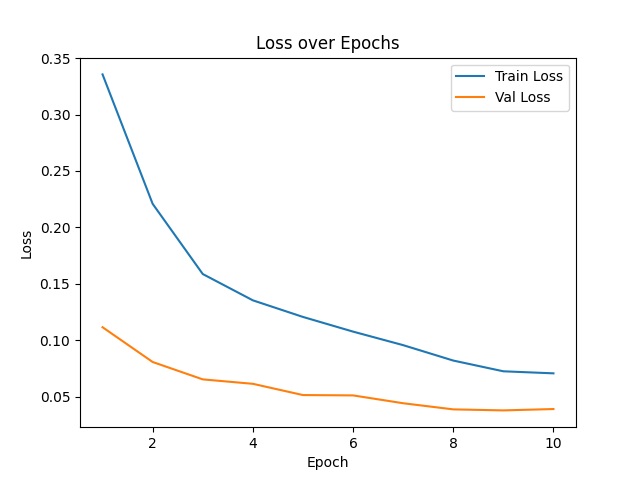
\includegraphics[width=\textwidth]{../../result/train_loss_attention.png}
        \caption{训练与验证集Loss变化曲线}
    \end{subfigure}
    \hfill
    \begin{subfigure}{0.45\textwidth}
        \centering
        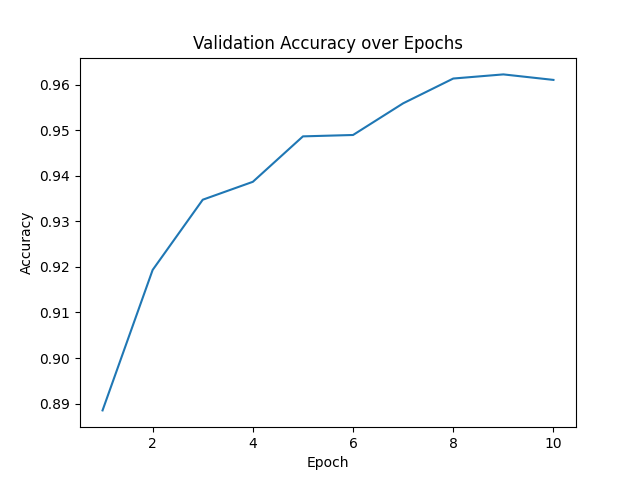
\includegraphics[width=\textwidth]{../../result/val_accuracy_attention.png}
        \caption{验证集Accuracy变化曲线}
    \end{subfigure}
    \caption{Attention 模型训练过程可视化}
\end{figure}

\begin{figure}[htbp]
    \centering
    \begin{subfigure}{0.45\textwidth}
        \centering
        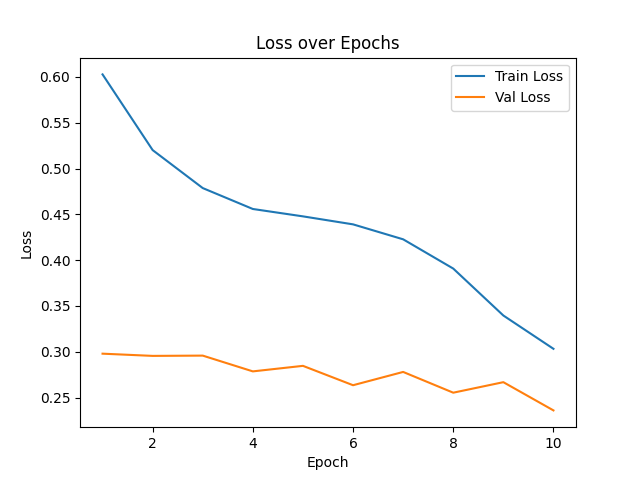
\includegraphics[width=\textwidth]{../../result/train_loss_rnn.png}
        \caption{训练与验证集Loss变化曲线}
    \end{subfigure}
    \hfill
    \begin{subfigure}{0.45\textwidth}
        \centering
        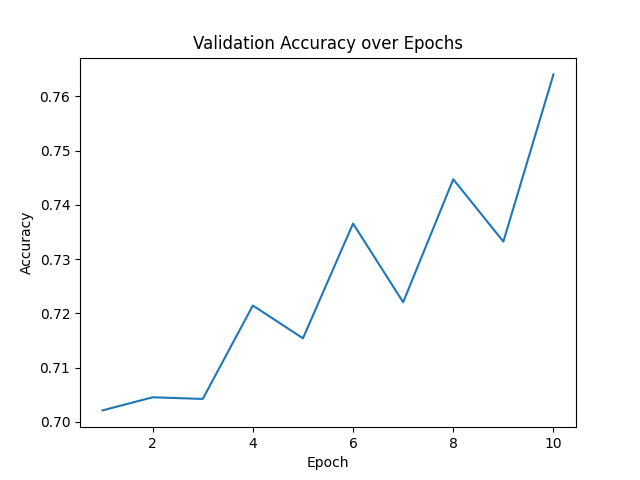
\includegraphics[width=\textwidth]{../../result/val_accuracy_rnn.png}
        \caption{验证集Accuracy变化曲线}
    \end{subfigure}
    \caption{RNN 模型训练过程可视化}
\end{figure}



\subsection{最终测试集性能}
\begin{table}[htbp]
\centering
\begin{tabular}{lcccc}
\toprule
模型 & Accuracy & Precision & Recall & F1-score \\
\midrule
Attention & 0.945 & 0.950 & 0.941 & 0.945 \\
RNN       & 0.766 & 0.792 & 0.731 & 0.760 \\
\bottomrule
\end{tabular}
\caption{Attention与RNN模型在Enron-Spam测试集上的性能对比}
\end{table}

\subsection{注意力机制可视化实验}
为加深理解, 使用\texttt{attention\_fig.py}脚本, 构造短序列并绘制其Self-Attention权重热力图:
\begin{figure}[htbp]
	\centering
	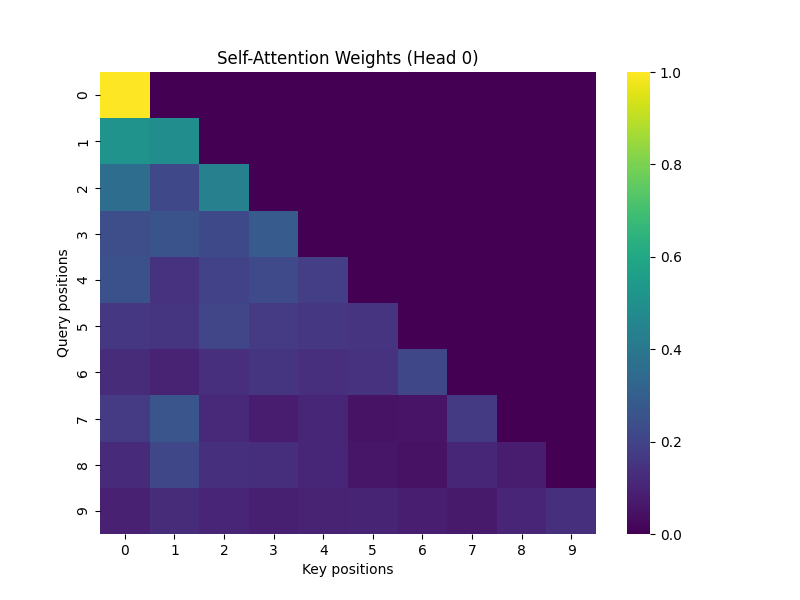
\includegraphics[width=0.5\textwidth]{../../result/attention_map.png}
	\caption{示例序列的Self-Attention权重热力图}
\end{figure}
可以观察到, 每个Token仅关注自身及其历史位置, 符合自回归Attention的建模逻辑.

\subsection{模型对比分析}
\subsubsection{模型性能对比}
Attention模型在准确率、Precision、Recall及F1-score等所有指标上均优于RNN, 主要归因于其更强的长距离依赖建模能力及丰富的表达特性.

\subsubsection{训练与推理效率}
尽管RNN单步计算开销较小, 但受限于时序依赖, 难以高效并行, 整体训练时间更长. 而Attention结构可充分利用并行计算资源, 训练速度明显更快, 推理阶段同样表现优异, 具备实际部署潜力.

\section{代码亮点总结}
\begin{itemize}
	\item \textbf{灵活的RNN模块设计}: 支持RNN/LSTM/GRU三种结构切换, 便于全面评估循环单元性能;
	\item \textbf{位置编码与因果掩码手动实现}: 加深了对Transformer内部原理的理解;
	\item \textbf{早停机制完备}: 即便本次未启用, 仍具备良好的工程规范;
	\item \textbf{模块化设计}: 训练、评估、可视化流程清晰分离, 代码可维护性与扩展性良好;
	\item \textbf{丰富的可视化支持}: 包括Loss、Accuracy、F1变化曲线与Attention热力图, 为训练过程监控与模型分析提供重要支撑.
\end{itemize}

\section{存在的局限性与改进建议}
\begin{itemize}
	\item \textbf{词表构建未引入预训练词向量}: 未来可结合GloVe、FastText等外部语义资源, 提升初始表示质量;
	\item \textbf{Attention结构较浅}: 目前仅使用单层Attention, 未来可探索堆叠多层、引入残差连接等策略;
	\item \textbf{Padding位置未屏蔽}: 建议在Attention中对\texttt{<pad>} Token添加mask, 减少无效注意力分配;
	\item \textbf{RNN变体评估不够全面}: 后续可系统对比RNN、LSTM、GRU在此任务下的细粒度性能差异;
	\item \textbf{推理效率缺乏定量评估}: 可进一步测试吞吐率、延迟等指标, 丰富推理阶段分析.
\end{itemize}

\section{结论与展望}
本实验充分展示了基于自注意力机制的模型在文本分类任务中的强大表现. 未来研究方向可包括:
\begin{itemize}
	\item 引入预训练Embedding或大规模预训练模型 (如BERT) 增强文本表示;
	\item 尝试旋转位置编码 (RoPE) 等先进位置编码方法;
	\item 深化模型层数, 引入多头注意力、残差与正则化策略, 提升模型泛化能力;
	\item 加强可解释性研究, 结合Attention可视化与梯度敏感性分析, 提高模型透明度与可控性;
	\item 探索小样本迁移学习与增量学习场景下的应用潜力.
\end{itemize}

未来的真正挑战, 在于兼顾性能、效率与可解释性, 推动深度学习模型向更加可持续、可信赖的方向演进.

\end{document}
